\documentclass{article}
\usepackage[T1]{fontenc}
\usepackage{lmodern}
\usepackage{graphicx}
\usepackage{amsmath,amssymb}
\usepackage[a4paper,margin=2cm]{geometry}
\usepackage[absolute,overlay]{textpos}
\setlength{\TPHorizModule}{1mm}
\setlength{\TPVertModule}{1mm}
\usepackage[indonesian]{babel}
\usepackage{hyperref}
\setlength{\emergencystretch}{2em}
% unit: Halaman 18

\begin{document}

% === Halaman 18 (python/native) ===

Penjelasan Analitik P + P = 2P = R

18

Persamaan tangen g:    y = mx + c

Gradien garis g: 𝑚= 𝑑𝑦

𝑑𝑥= 3𝑥𝑝2 + 𝑎

2𝑦𝑝

Perpotongan garis g dengan

 kurva: (mx + c)2 = x3 + ax + b

Koordinat Titik R: 

     xr = m2 – 2xp

     yr = m(xp – xr) – yp  

Jika yp = 0 maka m tidak terdefinisi

sehingga 2P = O

Sumber gambar: Andreas Steffen, 

Elliptic Curve Cryptography

% deskripsi: gambar native xref 90
\noindent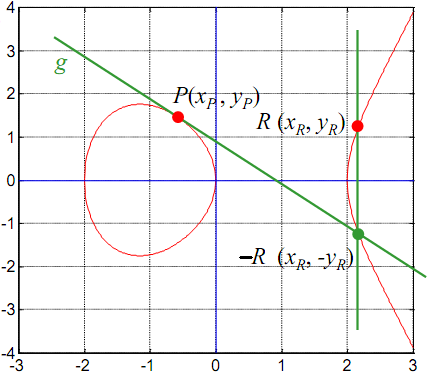
\includegraphics[width=0.85\textwidth]{../../images/python/page_018_img_01.png}

\end{document}
